\documentclass{beamer}

\usepackage[font=small,labelfont=bf]{caption}
\usepackage{longtable}
\usepackage{subfiles}
\usepackage{subfig}
\usepackage{booktabs}
\setlength{\tabcolsep}{6pt}
% \usepackage[table]{xcolor}
\title{Dual Optimization for Newsvendor-like Problem}
% \title{Dual Method for Solving Flight Mainte0.00ce Scheduling Problem}
\author{Chuwen}
\date{\today}

\begin{document}
\frame{\titlepage}



\begin{frame}
  \frametitle{FMP: variant case and weighted summation}
  \begin{align}
    \label{eq:fmp.obj}  f = & \min_{x_{it}, u_{it}, \delta_t, \epsilon_t}
    \textcolor{red}{b}^\mathsf{T}  \delta + \textcolor{red}{h}^\mathsf{T}\epsilon                                   \\
    \nonumber \mathbf{s.t.} &                                                                                       \\
    \label{eq:fmp.demand}   & \sum_i \textcolor{red}{c_i} u_{it} + \delta_t - \epsilon_t = d_t,\quad\forall t \in T \\
                            & U_{i, \cdot}, S_{i, \cdot}, X_{i, \cdot} \in \Omega_i,\quad \forall i\in I
  \end{align}
  \begin{itemize}
    \item \(b, h\) are time-variant
    \item \(c_i \neq 1\).
  \end{itemize}
\end{frame}


\begin{frame}
  \frametitle{FMP: Lagrangian relaxation}
  For the FMP, dual function:
  \[\begin{aligned}
      \phi(\lambda) & = - \sum_t \lambda_t d_t + \sum_i  \min_{\Omega_i} \textcolor{red}{c_i} \sum_t \lambda_t u_{it} \\
    \end{aligned}\]

  It reduces to a set of low dimensional minimization problems for each \(i \in I, \forall \lambda\)

  (Recall \(\lambda_t \in [-b, h] \) and \(\delta_t^\star = \epsilon_t^\star = 0\) else unbounded)
  \begin{equation}\label{subproblem}\begin{aligned}
      \min_{\Omega_i} \textcolor{red}{c_i} \sum_t \lambda_t \cdot u_{i,t}
    \end{aligned}\end{equation}
  \eqref{subproblem} is the subproblem to be solved by dynamic programming. (states: lifespan, action: work or start maintence)
\end{frame}

\begin{frame}
  \frametitle{FMP: subgradient method}
  At each iteration \(k\):
  \begin{itemize}
    \item  \(y_k\) solves \(\phi(\lambda_k) = \min_y \lambda_k^\mathsf{T}(y-b)\)
    \item for FMP: \(y_k = U_k ^\mathsf{T} \textcolor{red}{c}, U_k = (u^{(k)}_{it})\), solved from \eqref{subproblem} by DP.
    \item update \(\lambda_k\).
  \end{itemize}
\end{frame}
\begin{frame}
  \frametitle{Small case: \(|I| = 1, t = 2\) }
  \begin{align*}
    \textcolor{red}{c = 1} &                                                    & \textcolor{red}{c =2}                                                                                \\
    \min \quad             & 2\delta_0 + 3 \delta_1 + 4 \epsilon_0 + \epsilon_1 & \min \quad            & 2\delta_0 + 3 \delta_1 + 4 \epsilon_0 + \epsilon_1                           \\
    s.t. \quad             & u_0 + \delta_0 - \epsilon_0 = 1                    & s.t. \quad            & \textcolor{red}{2}u_0 + \delta_0 - \epsilon_0 = 1                            \\
                           & u_1 + \delta_1 - \epsilon_1 = 0                    &                       & \textcolor{red}{2}u_1 + \delta_1 - \epsilon_1 = 0                            \\
                           & 2 u_0 + s_0 = 6                                    &                       & 2 u_0 + s_0 = 6                                                              \\
                           & - 6 x_0 + 2 u_1 - s_0 + s_1 = 0                    &                       & - 6 x_0 + 2 u_1 - s_0 + s_1 = 0                                              \\
                           & x_0 + u_0 \le 1                                    &                       & x_0 + u_0 \le 1                                                              \\
                           & x_1 + u_1 \le 1                                    &                       & x_1 + u_1 \le 1                                                              \\
                           & s_0, s_1 \ge 2                                     &                       & s_0, s_1 \ge 2                                                               \\
    \textcolor{orange}{dual}                                                                                                                                                           \\
                           & -2 \le \lambda_0 \le 4                             &                       &                                                                              \\
                           & -3 \le \lambda_1 \le 1                                                                                                                                    \\
    \min_u                 & \lambda_0 (u_0 - 1) + \lambda_1 (u_1 - 0)          & \min_u                & \lambda_0 (\textcolor{red}{2}u_0 - 1)+ \lambda_1 (\textcolor{red}{2}u_1 - 0)
  \end{align*}

\end{frame}
\begin{frame}
  \frametitle{Small case: \(|I| = 1, t = 2\) }
  results:
  \begin{align*}
    \textcolor{orange}{gurobi:}                                      \\
    \textcolor{red}{c = 1} &       & \textcolor{red}{c =2}           \\
    u^\star = [1, 0]       & \quad & u^\star = [0, 0]                \\
    f^\star = 0            &       & f^\star = 2                     \\
    \textcolor{orange}{subgradient:}                                 \\
    \lambda_k = [-2, 0]    &       & \lambda_k = [-3.5203e^{-5},  0] \\
    \phi_k = 0             &       & \phi_k = 0                      \\
    u_k = [1, 0]           &       & u_k = [0, 0]                    \\
    \phi_k = f^\star       &       & \phi_k \neq f^\star
  \end{align*}

\end{frame}


\begin{frame}
  \frametitle{Small case, relax}
  results:
  \begin{align*}
    \textcolor{orange}{gurobi:  u \in [0, 1]    }          \\
    \textcolor{red}{c = 1} &       & \textcolor{red}{c =2} \\
    u^\star = [1, 0]       & \quad & u^\star = [0.5, 0]    \\
    f^\star = 0            &       & f^\star = 0           \\
    \textcolor{orange}{gurobi:    x \in [0, 1]      }      \\
    \textcolor{red}{c = 1} &       & \textcolor{red}{c =2} \\
    u^\star = [1, 0]       & \quad & u^\star = [0, 0]      \\
    f^\star = 0            &       & f^\star = 2           \\
  \end{align*}
\end{frame}

\begin{frame}
  \frametitle{Small case}

  The subgradient method (sg) stops at (maximum) 400 iterations, then compared with benchmarks by Gurobi (grb).
  \begin{itemize}
    \item lb\_grb, \(f_{\textsf{grb}}\)  are lower bound, primal value from grb.
    \item \(f^u_{\textsf{relax}}, f^x_{\textsf{relax}}\) primal value from grb for problem with \textcolor{red}{relaxed \(u\) and \(x\) only}, respectively: \textcolor{red}{\(f^x_{\textsf{relax}} = f^\star\) ?}
    \item t\_grb, t\_sg are runtime from grb and sg, respectively.
    \item \(\phi_{\textsf{sg}}\) is the dual value (\(\phi\)) by sg.
    \item \(z_{\textsf{sg}}\) is primal value in sg using averaged primal recovery, i.e.
          \[z_{\textsf{sg}} = z(\bar y_k) = f(\bar \delta_k, \bar \epsilon_k)\]
    \item \(\phi_{\textsf{gap}}\), z\_gap are relative gap from sg to grb for dual and primal values.
  \end{itemize}
\end{frame}

\begin{frame}
  \frametitle{FMP: \(c=1\) small case \(5\times 5\)}
  \scriptsize
  \begin{tabular}{lllrrrrrlllll}
    \toprule
    {} & lb\_grb                  & \(f_{\textsf{grb}}\)     & t\_grb
       & \(f^u_{\textsf{relax}}\) & \(f^x_{\textsf{relax}}\)
       & t\_sg                    & \(\phi_{\textsf{sg}}\)   & \(\phi_{\textsf{gap}}\)                                             \\
    %  & \( z_{\textsf{sg}}\) & z\_gap                                                                    \\
    \midrule
    0  & 34.00                    & 34.00                    & 0.01                    & 32.50  & 34.00  & 1.26 & 34.00  & 0.00\%  \\
    1  & 42.00                    & 42.00                    & 0.01                    & 40.83  & 42.00  & 0.01 & 42.00  & 0.00\%  \\
    2  & 84.00                    & 84.00                    & 0.01                    & 78.25  & 84.00  & 0.01 & 84.00  & 0.00\%  \\
    3  & 49.00                    & 49.00                    & 0.01                    & 45.50  & 49.00  & 0.04 & 48.96  & -0.08\% \\
    4  & 50.00                    & 50.00                    & 0.01                    & 50.00  & 50.00  & 0.00 & 50.00  & 0.00\%  \\
    5  & 112.00                   & 112.00                   & 0.01                    & 106.17 & 112.00 & 0.01 & 112.00 & 0.00\%  \\
    6  & 47.00                    & 47.00                    & 0.02                    & 47.00  & 47.00  & 0.02 & 47.00  & 0.00\%  \\
    7  & 69.00                    & 69.00                    & 0.03                    & 67.33  & 69.00  & 0.04 & 68.98  & -0.04\% \\
    8  & 41.00                    & 41.00                    & 0.02                    & 34.25  & 41.00  & 0.64 & 41.00  & 0.00\%  \\
    9  & 91.00                    & 91.00                    & 0.00                    & 89.67  & 91.00  & 0.01 & 91.00  & 0.00\%  \\

    \bottomrule
  \end{tabular}
  \normalsize
\end{frame}

\begin{frame}
  \frametitle{FMP: \(c = 1\) large case \(10\times 15\)}

  \begin{itemize}
    \item \(f^x_{\textsf{relax}} \neq f^\star\)
  \end{itemize}


  \scriptsize

  \begin{tabular}{lllrrrlllll}
    \toprule
    {} & lb\_grb                  & \(f_{\textsf{grb}}\)     & t\_grb
       & \(f^u_{\textsf{relax}}\) & \(f^x_{\textsf{relax}}\)
       & t\_sg                    & \(\phi_{\textsf{sg}}\)   & \(\phi_{\textsf{gap}}\)                                             \\
    %  & \( z_{\textsf{sg}}\) & z\_gap                                                                    \\
    \midrule
    0  & 467.00                   & 467.00                   & 0.59                    & 460.25 & 455.00 & 3.97 & 467.00 & 0.00\%  \\
    1  & 375.00                   & 375.00                   & 0.22                    & 370.00 & 366.00 & 0.12 & 375.00 & 0.00\%  \\
    2  & 158.00                   & 158.00                   & 0.67                    & 155.92 & 158.00 & 4.73 & 158.00 & 0.00\%  \\
    3  & 463.00                   & 463.00                   & 0.80                    & 457.08 & 458.00 & 5.86 & 463.00 & 0.00\%  \\
    4  & 370.00                   & 370.00                   & 0.11                    & 367.17 & 363.00 & 4.46 & 370.00 & 0.00\%  \\
    5  & 336.00                   & 336.00                   & 1.04                    & 329.17 & 333.00 & 0.10 & 336.00 & 0.00\%  \\
    6  & 350.00                   & 350.00                   & 0.74                    & 344.42 & 348.00 & 3.93 & 350.00 & 0.00\%  \\
    7  & 416.00                   & 416.00                   & 0.09                    & 409.17 & 409.00 & 0.19 & 415.61 & -0.09\% \\
    8  & 374.00                   & 374.00                   & 0.88                    & 363.50 & 363.00 & 7.81 & 374.00 & 0.00\%  \\
    9  & 343.00                   & 343.00                   & 1.30                    & 330.67 & 336.00 & 0.24 & 342.67 & -0.10\% \\
  \end{tabular}
  \normalsize


\end{frame}

\begin{frame}
  \frametitle{FMP: \(c = 1\) large case \(10\times 15\), primal solution}
  \(z_k\) is the value of best primal (recovery) solution,
  \(\phi_k\) is the dual value, \(f^\star\) is the benchmark optimal value by grb.
  \textcolor{red}{there is a gap from \(z_k\) to \(f^\star\)}
  \begin{figure}

    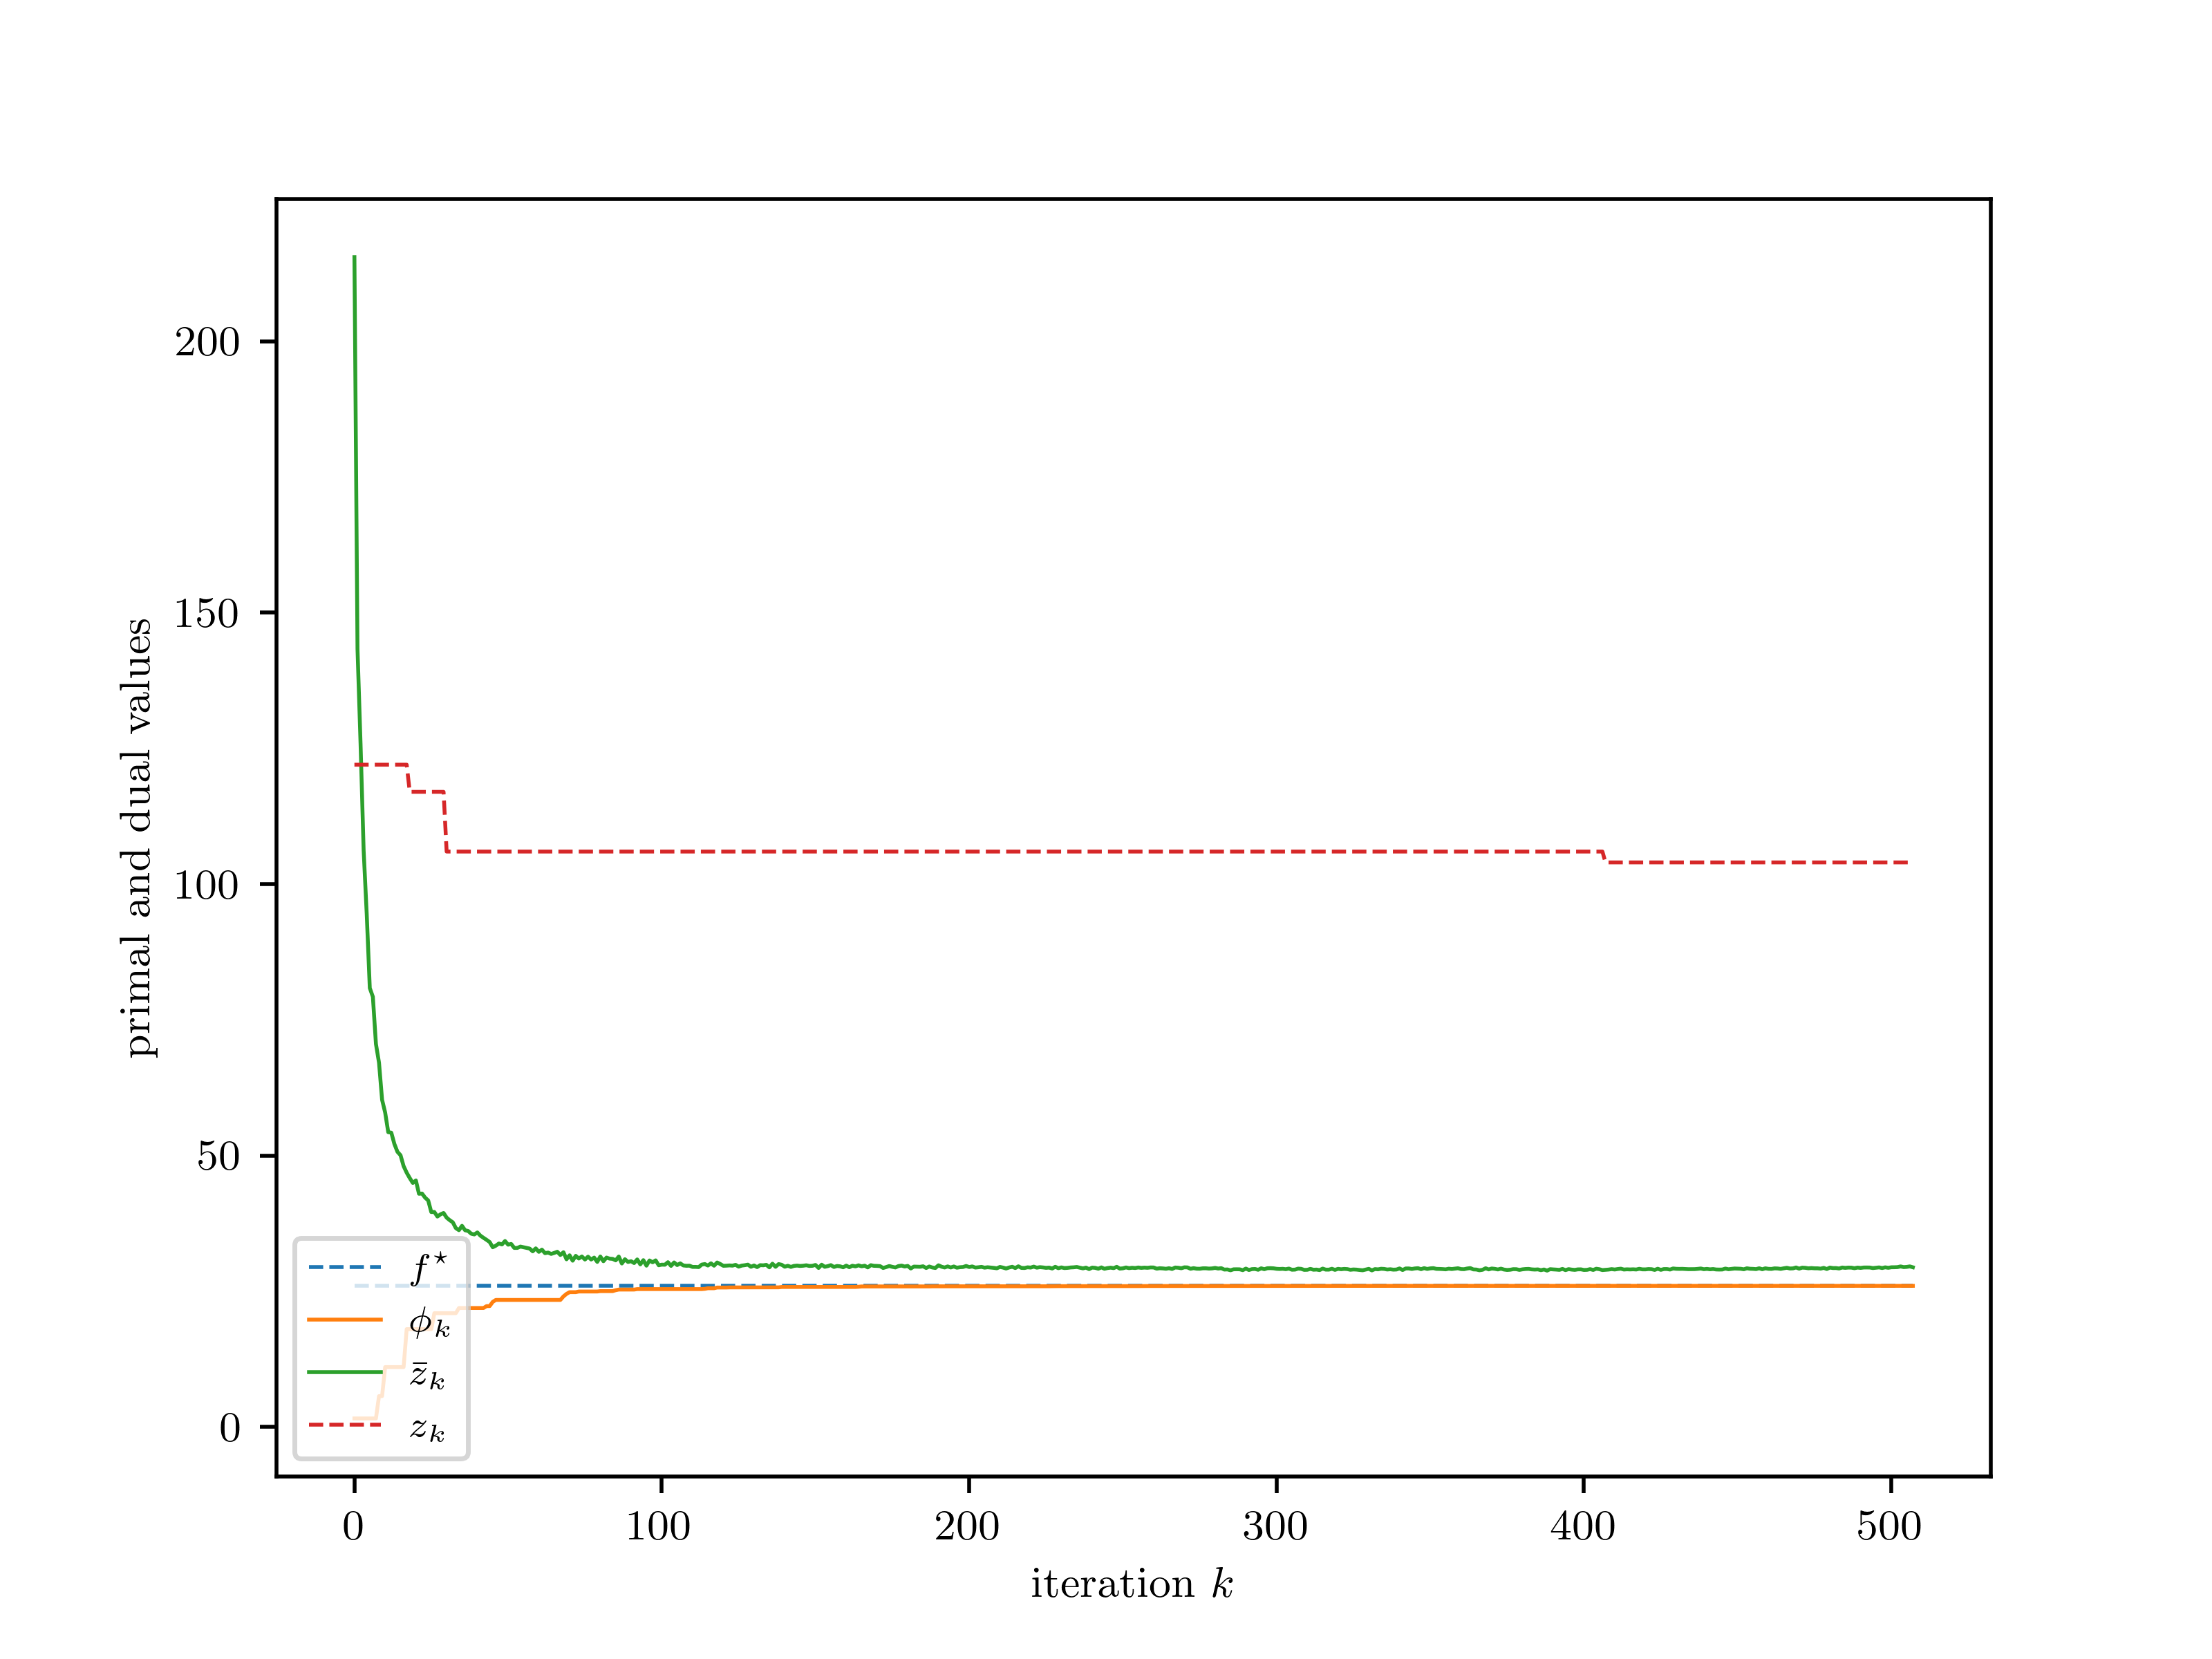
\includegraphics[width=.89\linewidth]{imgs/conv_0_normal_sg_10_15.png}

    \label{fig:divergent_volume}
  \end{figure}
\end{frame}

\begin{frame}
  \frametitle{FMP: \(c \neq 1\) small case \(5 \times 5\)}
  \scriptsize
  \begin{tabular}{lllrrrlllll}
    \toprule
    {} & lb\_grb                  & \(f_{\textsf{grb}}\)     & t\_grb
       & \(f^u_{\textsf{relax}}\) & \(f^x_{\textsf{relax}}\)
       & t\_sg                    & \(\phi_{\textsf{sg}}\)   & \(\phi_{\textsf{gap}}\)                                           \\
    %  & \( z_{\textsf{sg}}\) & z\_gap                                                                                                                                      \\
    \midrule
    0  & 8.00                     & 8.00                     & 0.01                    & 0.00  & 8.00  & 0.75 & -0.00 & -99.99\% \\
    1  & 9.00                     & 9.00                     & 0.01                    & 0.00  & 9.00  & 0.68 & 8.00  & -11.11\% \\
    2  & 55.00                    & 55.00                    & 0.02                    & 52.50 & 55.00 & 1.33 & 54.98 & -0.03\%  \\
    3  & 11.00                    & 11.00                    & 0.03                    & 5.00  & 11.00 & 1.06 & 10.00 & -9.09\%  \\
    4  & 7.00                     & 7.00                     & 0.02                    & 0.00  & 7.00  & 0.85 & 4.00  & -42.85\% \\
    5  & 20.00                    & 20.00                    & 0.03                    & 12.33 & 20.00 & 1.08 & 20.00 & -0.00\%  \\
    6  & 22.00                    & 22.00                    & 0.01                    & 20.00 & 22.00 & 0.01 & 22.00 & 0.00\%   \\
    7  & 15.00                    & 15.00                    & 0.01                    & 8.67  & 15.00 & 0.01 & 15.00 & 0.00\%   \\
    8  & 14.00                    & 14.00                    & 0.03                    & 6.00  & 14.00 & 1.01 & 10.00 & -28.57\% \\
    9  & 18.00                    & 18.00                    & 0.02                    & 13.00 & 18.00 & 0.68 & 18.00 & -0.00\%  \\
    \bottomrule
    \normalsize
  \end{tabular}
\end{frame}

\begin{frame}
  \frametitle{Conclusion}

  \begin{itemize}
    \item ? zero duality gap: \(\phi^\star = f^\star\), \(\phi^\star\) is the best bound by \(\phi\) and \( f^\star\) is the best primal value.
    \item ? can we bound the quality of heuristic for averaged solution? \(\bar z_k = z(\bar y_k)\) converges to \(\phi^\star\):
          \[|\bar z_k - \phi^\star| \]
    \item ? can we improve \(\bar z = z(\bar y)\), round \(\bar z\)
  \end{itemize}
\end{frame}

\end{document}
